\documentclass {article}
\usepackage[utf8]{inputenc}
\usepackage[english]{babel}
\usepackage{fancyhdr}
 
\pagestyle{fancy}
\usepackage{fancyheadings}
\pagestyle{fancy}
\rhead{David Ram\'irez P\\Tarea 2\\Teor\'ia de Aut\'omatas}



\usepackage {tikz}
\usepackage{pgf}
\usetikzlibrary{arrows,automata}
\usetikzlibrary {positioning}
%\usepackage {xcolor}
\definecolor {processblue}{cmyk}{2,0,0,0}
\begin {document}
Ejercicio 2
\begin {center}
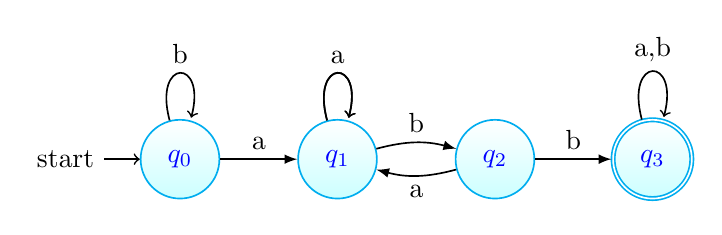
\begin{tikzpicture}[-latex ,auto ,node distance =2 cm and 2cm ,on grid ,
semithick ,
state/.style ={ circle ,top color =white , bottom color = processblue!20 ,
draw,processblue , text=blue , minimum width =1 cm}]
\node[state, initial] (q0) {$q_0$};
\node[state, right of=q0] (q1) {$q_1$};
\node[state, right of=q1] (q2) {$q_2$};
\node[state, accepting, right of=q2] (q3) {$q_3$};
\draw (q1) edge[loop above] node{a} (q1)
(q0) edge[loop above] node{b} (q0)
(q0) edge[above] node{a} (q1)
(q1) edge[loop above] node{} (q1)
(q1) edge[bend left =15, above] node{b} (q2)
(q2) edge[below,bend left =15] node{a} (q1)
(q2) edge[above] node{b} (q3)
(q3) edge[loop above] node{a,b} (q3)
;

\end{tikzpicture}
\end{center}
\end{document}